\documentclass[11pt]{article}

%----------- conforms to NSF specs
\setlength{\topmargin}{-13mm}
\setlength{\oddsidemargin}{1mm}
\setlength{\textwidth}{164mm}
\setlength{\textheight}{228mm}
%-----------

\addtolength{\parskip}{+.2\baselineskip}

\usepackage{graphicx,url}
\usepackage{amsmath,alltt,xspace,theorem}
\newcommand{\BA}{{B\"{u}chi automata}\xspace}
\thispagestyle{empty}


\begin{document}
 
  \begin{center}
  {\Large\bf  {CS 6110, Spring 2022} } \\
  {\bf Description of a Distributed Locking Protocol} \\
  {Class Handout for Lecture 8, 2/3/2022}
  \end{center}

\section{Introduction}
\label{sec:introduction}

\begin{figure}[tbhp]
\centering
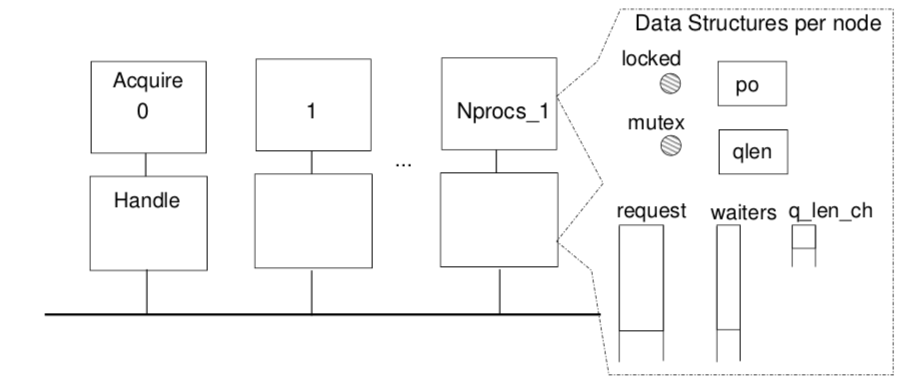
\includegraphics[scale=0.4]{fig1.png}
 \caption{The Architecture of a Distributed Locking Protocol}
 \label{fig:locking-prot-arch}
\end{figure}
%
\begin{figure}[tbhp]
\centering
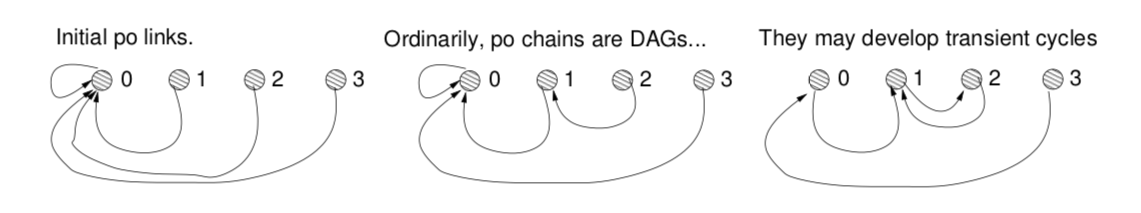
\includegraphics[scale=0.4]{fig2.png}
 \caption{The {\tt po} DAG, and also transient cycles that can form}
 \label{fig:locking-prot-cycles}
\end{figure}
%
A distributed locking protocol (``locking protocol'') is our
subject of study in Assignment 3.
%
This protocol is an abstraction of an actual protocol employed in the Quarks
software distributed shared memory system developed at Utah by Mr. Dilip Khandekar (MS, Utah, 1995) and
Prof. John Carter (now Dr. John Carter, distinguished
researcher at IBM) around 1995 \footnote{D. Khandekar, {\em Quarks: Portable Distributed
    Shared Memory on Unix}, Computer Systems Laboratory, University of
  Utah, 1995.}
%
We could imagine the lock being a comfortable chair on which only one
person can sit at a time, and the participating processes
are a collection of people who want to serially reuse the chair.
%
Initially, process 0 possesses the chair and may, at will, sit on it zero
or more times in succession.
%
When a process sits on the chair, it sets a variable {\tt locked} to 1;
when it is not, it sets the variable to 0.
%
Initially every other process knows who the current owner of the chair is: namely
process 0.
%
They indicate this through a variable called ``probable owner'' ({\tt po}).
%
Figure~\ref{fig:locking-prot-arch} shows the architecture of the system
while
Figure~\ref{fig:locking-prot-cycles} shows the kinds of {\tt po} cycles that
can develop during this protocol.
%
The initial situation with {\tt po} chains is shown left-most in 
Figure~\ref{fig:locking-prot-cycles}, where
every process has {\tt po = 0}, and in this case the ``probable owner''
is also the actual owner.
%
Later on, as the protocol executes, the probable owner is not going to be the actual
owner.
%
In quiescent states, the {\tt po} chains form a directed acyclic graph (DAG) with
the sink node being the actual lock owner, as
in the middle of Figure~\ref{fig:locking-prot-cycles}.
%
However, as shown in the right-hand side of
Figure~\ref{fig:locking-prot-cycles}, we may even have transcient cycles develop,
and these may persist for an arbitrary number of steps, as will be very soon
illustrated when we discuss the details of this protocol.

To model reality a bit more, each process is split into an {\tt acquire}
thread and a {\tt handle} thread.
%
The {\tt acquire} thread is the main thread. In a perpetual loop, it
does the following things:
%-----------------------------------------------------------------
\begin{itemize}
\item If the chair isn't available, request it,
  and wait; when woken up, the chair is available;
\item Now that the chair is
  available, make sure that {\tt locked} is set to 1,
  sit on the chair and relax for a while;
\item Now see if there are a queue of waiters for the chair; if
  not, just set {\tt locked} to 0, and repeat this loop; else,
  let the queue of waiters be {\tt h::t} where {\tt h} is the
  head waiter and {\tt t} the tail of the queue. Send the chair
  to {\tt h}, passing along {\tt t} also to it.
\end{itemize}
%-----------------------------------------------------------------

The {\tt handler} thread is a helper thread. In a perpetual loop, it
does the following things:
%-----------------------------------------------------------------
\begin{itemize}
\item Wait for an incoming message to arrive at node $i$'s handler.
\item If {\tt po} is pointing to another node $j$, pass the message along to $j$.
\item If {\tt po} is pointing to $i$, and the lock is currently free
   (it is 0 currently),
   {\em it is a {\bf likely invariant} that the queue of waiters at this node is empty}.
   Then, we simply send the lock (``the chair'') to the requesting process.
\item Finally, if
  {\tt po} is pointing to $i$, and the lock is not currently free (it is 1 currently),
  then we simply queue up the requester into the queue of waiters.
  It will be ensured that this queue of waiters will be later processed by
  proctype {\tt acquire} when it eventually frees up the lock.
\end{itemize}
%
\begin{figure}[tbhp]
\centering
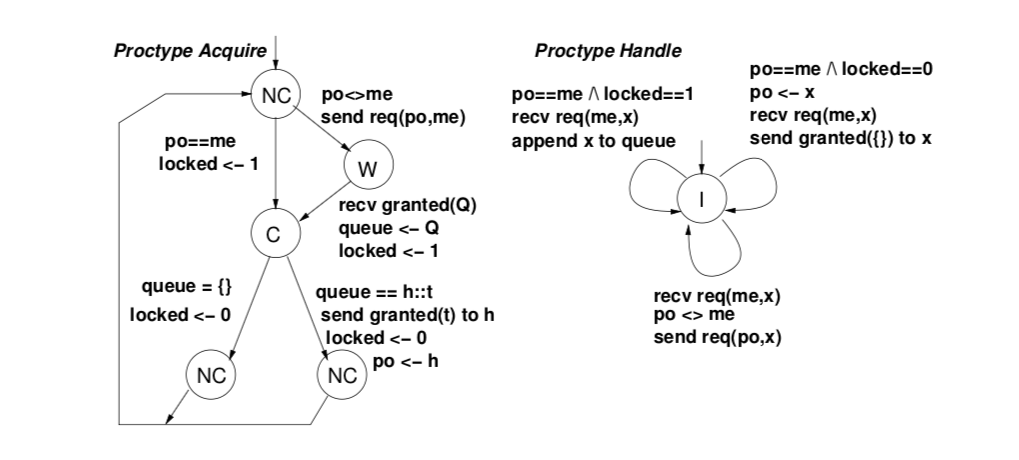
\includegraphics[scale=0.4]{fig3.png}
 \caption{The State Machines}
 \label{fig:locking-prot-sm}
\end{figure}
%
The finite state machines in Figure~\ref{fig:locking-prot-sm}
describe these steps more concretely.

A few protocol scenarios will help solidify the understanding of
this protocol
in the reader's minds.
%
Consider how the cycle in Figure~\ref{fig:locking-prot-cycles} middle
can develop starting from the initial {\tt po} graph shown on the left.
%
Consider the sequence of lock acquisitions: P1 gets the lock, then P2
gets the lock, then P1 gets the lock, and finally P0 gets the lock.
%-----------------------------------------------------------------
\begin{itemize}
\item When P1 requests P0 and obtains the lock, P0's {\tt po} pointer
  is adjusted to point to P1, and P1 would point to itself.
\item P2's {\tt po} variable would still be pointing to P0. Therefore,
  when P2 requests the lock, the request would initially go to P0
  which would pass along the request to P1. P1 would grant the lock to P2,
  while updating its PO variable to P2. When P2 receives the lock, it sets
  its {\tt po} variable to point to itself.
\item Now P1 requests the lock and obtains it back; the end result
  would be one where P2 points to P1 and P1 points to itself, while
  P0 points to P1. In this hand-over, there would be a transient
  graph cycle as shown in the right-hand side of
  Figure~\ref{fig:locking-prot-cycles}.
  The end result would of course be the DAG shown in the middle
  of Figure~\ref{fig:locking-prot-cycles}.
\end{itemize}
%--


% Promela also...SMV query can back-justify and calculate this
% Testing connection...

\section{Data Structures}
\label{sec:ds}
%
Figure~\ref{fig:locking-prot-sm} shows the {\tt acquire} and {\tt handle}
state machines.
%
We will now describe how these state machines act on the data structures
shown in Figure~\ref{fig:locking-prot-arch}.
%
There is one bit {\tt locked} held at every {\tt acquire} process.
%
A mutex {\tt mutex} protects shared accesses between {\tt acquire}
and {\tt handle}.
%
Variable {\tt po} maintains the probable owner information.
%
A queue of length 1 called {\tt q\_len\_ch} is maintained.
%
This queue is used to convey the {\em number} of waiters that are
going to be forwarded to this node.
%
The actual waiters themselves are going to be sent separately, and
they arrive into the {\tt waiters} queue which is of
size {\tt Nprocs\_1} ({\tt Nprocs - 1}).
%
{\em This is a commonly used protocol design approach} because
sending advanced notification of how many are to arrive often
helps prepare the receiving process for the burst of arrivals.
%  
Variable {\tt qlen} records the number of waiters in the
queue {\tt waiters}.
%
Finally, there is also a queue {\tt request} also of
size {\tt Nprocs\_1} into which incoming requests arrive.

It is sufficient for the size of the {\tt waiters} and {\tt request} 
queues to be one less than the number of
processes ({\tt Nprocs\_1}), 
because of two (related) reasons: (i)~the number of waiters at
any time cannot be more than this number, and
(ii)~the case of a process that owns the lock and
sends a request to itself does not arise (and so, allocating 
{\tt Nprocs} locations is wasteful).
%
Notice that this allocation is {\em still} excessive in two respects:
%
\begin{itemize}
\item Since there can be at-most {\tt Nprocs\_1} requests in the
  system at any time, most of the buffer locations will be unoccupied.
\item Since the buffering needs grow quadratically,
  the overall design can be very expensive
  if {\tt Nprocs} is large.
\end{itemize}
%
We shall later study changes to the protocol to arrive at a more
economical implementation in terms of buffering needs.
%
For the present protocol, however, we shall have to be content with
allocating $O(Nproc^2)$ buffer locations.

\section{Promela Coding}

Salient aspects of the Promela code will now be discussed.

First, we begin with a few constants and type synonyms:
%
\begin{small}
\begin{verbatim}
#define Nprocs 4
#define Nprocs_1 3

#define PID byte
\end{verbatim}
\end{small}

The data structures described in Section~\ref{sec:ds} are
declared below:
%
\begin{small}
\begin{verbatim}
bit mutex[Nprocs];
PID po[Nprocs];
chan request[Nprocs] = [Nprocs_1] of {PID};
chan q_len_ch[Nprocs] = [1] of {byte};
chan waiters[Nprocs] = [Nprocs_1] of {PID};
byte qlen[Nprocs];   /* How many are waiting? */
bit locked[Nprocs];
\end{verbatim}
\end{small}

A variable is declared to be able to state properties:
\begin{small}
\begin{verbatim}
byte pid_acq[Nprocs]; /* PID of acquire process  */
\end{verbatim}
\end{small}

The actions of {\tt acquire} are now described beginning with
lock acquisition.
%
\noindent$\bullet$
First we take the {\tt mutex} that controls accesses
between {\tt acquire} and {\tt handle}
\begin{small}
\begin{verbatim}
        atomic { mutex[me] == 0 ->  
                 mutex[me] = 1 };
\end{verbatim}
\end{small}

\noindent$\bullet$
Next, if {\tt po[me]==me}, process `{\tt me}' can acquire the lock.
Else, through {\tt request[po[me]]!me}, we send a request to
who `{\tt me}' thinks to be the probable owner.
%
The request itself consists of {\tt me}, i.e., the sending processes's ID.

\noindent$\bullet$
We then release the {\tt mutex} and wait for the condition
%
\begin{small}
\begin{verbatim}
  q_len_ch[me] ? [count] && mutex[me]==0
\end{verbatim}
\end{small}
%
This says that something has arrived in the {\tt q\_len\_ch} channel.
%
This condition is tested as the {\em guard} of an {\tt atomic}
and hence  we are able to take {\tt mutex} also in this case.

\noindent$\bullet$
The next section of code is very interesting:
%
\begin{small}
\begin{verbatim}
                                po[me] = me;
                                mutex[me] = 1;
                                q_len_ch[me] ? count;
                                        assert(qlen[me]==0);
                                qlen[me] = qlen[me]+count;
                                count = 0
                        };
                        ( len(waiters[me]) == qlen[me] );
                        locked[me] = 1;
                        mutex[me]=0
\end{verbatim}
\end{small}
We first set {\tt me} to be the probable ownewr, thus owning the lock.
Note that this is another way of recording that a lock is acquired
(other than explicitly setting {\tt locked}, which happens towards
the end of this code fragment).
%
In many protocols, we will find such variables that approximately
track each other, and yet may subtly differ in semantics.
%
For instance, in the present situation, we set {\tt po[me] = me}
as soon as we know the count of waiters being forwarded.
%
We will set {\tt locked[me] = 1} only after the waiters have arrived.
%
It is possible to `enjoy' the lock after the first event itself.
%
However, in some protocols, it may make an observable difference as
to when we start enjoying the lock.

\noindent$\bullet$
We obtain the count of the number of messages
yet to arrive on the {\tt waiters} queue via
{\tt q\_len\_ch[me] ? count}.
%
We also sanity-check our code through the
{\tt assert} statement {\tt assert(qlen[me]==0)}.
%
This means that there ought to be nothing accumulated in the
{\tt waiters} queue locally.
%
This is of course correct, since proctype {\tt me} just now
acquired the lock, and so there was no possibility of it
accumulating arriving requests in the {\tt waiters} queue.
%
In particular, the code of {\tt handler} shows that if the lock
is {\em not} held in the local site, then arriving requests
are forwarded along the {\tt po} chain.
%
Thus, we do {\tt assert(qlen[me]==0)} and then
safely accumulate {\tt count} via {\tt qlen[me] = qlen[me]+count}.
%
We perform {\tt count=0} as a manual `dead variable' elimination step.
%
Then, {\tt ( len(waiters[me]) == qlen[me] )} is a statement that
blocks till the expected number of waiters have all arrived.
%
Finally we do {\tt locked[me]=1} and {\tt mutex[me]=0}; the latter
step now allows the {\tt handler} thread to run.

\noindent$\bullet$
Releasing the lock is interesting. We acquire the mutex, and in
the same step do {\tt locked[me]=0}.
\begin{small}
\begin{verbatim}
    release:
        atomic {
            mutex[me] == 0 ->
            locked[me] = 0;
            mutex[me] = 1
        };
\end{verbatim}
\end{small}

\noindent$\bullet$
We now iterate till {\tt qlen[me]} drops to 0.
Notice how we set {\tt po[me]} directly from the
head of {\tt waiters[me]}. Notice how we also send
the one-diminished number of waiters in {\tt q\_len\_ch}.
The last {\tt assert} uses \verb|>=|; it could truly be
\verb|=|.
%
Even though further requests might arrive after
{\tt mutex[me] = 0}, they will promptly be forwarded
and not stored, becuase we've already updated our {\tt po[me]}.
%
\begin{small}
\begin{verbatim}        
        if
        :: qlen[me] ->
            waiters[me] ? po[me];
            qlen[me] = qlen[me]-1;
            q_len_ch[po[me]] ! qlen[me];
            do
            :: qlen[me] -> atomic {
                waiters[me] ? thread;
                waiters[po[me]] ! thread;
                thread = 0;
                qlen[me] = qlen[me]-1
               }
            :: !qlen[me] -> break
            od
        :: !qlen[me] -> skip
        fi;
        mutex[me] = 0;
        assert (qlen[me] >= 0);
    goto loop
\end{verbatim}
\end{small}

\noindent$\bullet$
proctype handle employs
the guard {\tt mutex[me] == 0 \&\& request[me]?[requester]} and
acquires the {\tt mutex}, and also obtains the
requester via {\tt request[me]?requester}.
%
The rest of its actions are self-explanatory.
%
\begin{small}
\begin{verbatim}        
proctype handle(int me)
{
    PID requester;
    do
    :: atomic {
            mutex[me] == 0 && request[me]?[requester]
                 ->
            mutex[me] = 1;
            request[me] ? requester
        };
        if
        :: po[me] != me -> request[po[me]] ! requester
        :: po[me] == me && locked[me] ->
                    waiters[me] ! requester;
                    qlen[me] = qlen[me] + 1;
                    assert (qlen[me] < Nprocs)
        :: po[me] == me && !locked[me] ->
                    q_len_ch[requester] ! 0;
                    assert (qlen[me] == 0);
                    po[me] = requester
        fi;
        mutex[me] = 0
    od
}
\end{verbatim}
\end{small}

\noindent$\bullet$ We spawn the right number of processes:
\begin{small}
\begin{verbatim}  
init {
    byte cnt;

    atomic {
        do
        :: cnt == Nprocs-> break
        :: cnt != Nprocs->
                      pid_acq[cnt] = run acquire(cnt);
                      run handle(cnt);
                      cnt = cnt+1
        od
    }
}
\end{verbatim}
\end{small}

\subsection{Verification}

As far as the properties of interest go,
one can state the obvious safety property that the lock
can be held in exactly one place at any time.
%
There are many more safety and liveness properties that
we don't discuss, but encourage the reader to think about.
%
In particular, think about how transient cycles might affect
the correctness of things you state.
%
A natural fairness condition to employ would be that eventually
the transient cycles will go away (a function of scheduling).

We tried verifying the following liveness property:
\begin{small}
\begin{verbatim}
#define at_release_0   (acquire[pid_acq[0]]@release)
#define at_release_1   (acquire[pid_acq[1]]@release)
#define at_release_2   (acquire[pid_acq[2]]@release)
#define at_release_3   (acquire[pid_acq[3]]@release)
/*
 * Formula As Typed:
     ([]  <>  at_release_0) || ([]  <>  at_release_1)
  || ([]  <>  at_release_2) || ([]  <>  at_release_3)
 * The Never Claim Below Corresponds. ....
 */
\end{verbatim}
\end{small}
The LTL to B\"{u}chi automaton translator obtains a rather impressive
looking automaton, and the property was found violated.

\subsection{Tasks of interest}

\noindent One can/must do these steps:
\begin{enumerate}
\item In Asg3 you are asked to verify the
  buggy protocol, explaining the bug and the fix
\item Answer the random PO idea suggested there
\end{enumerate}

\end{document}

